\openepigraph{The secret to multitasking is that it isn't actually multitasking. It's just extreme focus and organization.
}{---Joss Whedon}


In the second mini-project, you will read, summarize and discuss the paper by \citeauthor{stoet_are_2013} (2013)\cite{stoet_are_2013}. Then, you will attempt to replicate their results in the lab, by conducting an experiment and analyzing the data.

\section{What's in store}

\begin{enumerate}
\item Students read paper and write QALMRI (15-20)
\item Group discussion about paper (15-20)
\item Students download the task-switching program available from the website and individually complete the task. Individual students then enter their data in the master spreadsheet
\item Discussion of how to analyze the data. Major analysis goals are:

a.	Was there a mixing cost? Compare pure lists to mixed lists

b.	Was there a switching cost? Compare switch vs. repeat trials in pure lists

c.	Did these effects depend on gender? Did the women have a smaller mixing cost than the men? Did the women have a smaller switching cost than the men?

\item Students break into groups to analyze the data.

\end{enumerate}

\section{Critical Concepts}

\subsection{Multiple Dependent and Independent Variables}

In lab 5 we begin looking at more complex designs that involve multiple dependent or and independent variables. For example, we can look at the dependent variable of reaction time or error rate, which are our two difference measured variables. There are also three independent variables, including gender (male vs female), block (pure list vs. mixed list), and trial sequence (repeat trial vs. switch trial). 

\subsection{Main effects and interactions}
Throughout this course we will be talking a lot about main effects and interactions. Feel free to jump ahead in the textbook and learn more about them. 

Main effects refer to the influence of single independent variables. And, each independent variable always has one main effect. So, we could look at the main effect of gender, block, or trial sequence. The main effect is like conducting a one-way ANOVA on the variable of interest, collapsing over the other variables. For example, a main effect of trial sequence usually shows slower mean reaction times in the switch condition compared to the repeat condition. This is called the task-switching cost, or also the task-switching effect.

Interactions occur when the effect of one independent variable depends on the levels of another independent variable. For example, if women actually multi-task better than men, then we should expect an interaction between gender and task-switching. Specifically, women should be better at task-switching than men. This would mean that women should have smaller task-switching costs (meaning they are unaffected by switching) compared to men (who should have bigger task-switching costs if they are more affected by switching).

If women have smaller task switching costs than men, then the effect of task-switching independent variable (repeat vs. switch) will depend on the level of the gender variable (women vs. men), which is the definition of an interaction.

\subsection{Manipulating an Effect}

Things get complicated when we add more dependent and independent variables, and it can be easy to lose track of what is going on in an experiment.

Many experiments are conducted for the purpose of better understanding some phenomena. For example, researchers observe phenomena like the task-switching effect, they create theories to explain the phenomena, then they test their theories by running more experiments. 

A primary question is often to identify factors that manipulate, influence, or somehow change the phenomena of interest. We know that switching between tasks can hurt performance, and we measure this cost by calculating a switch cost, which is the difference in performance between switching conditions and repeating conditions. What kinds of factors would make this cost ? Perhaps extended practice, time of day, gender, personality, motivation, drug interventions, details of the task, and many other factors could make the normal cost get smaller. Many of these factors might also make the effect get larger. And, knowledge of what makes switching costs smaller or larger can be used to test theories, which need to explain how and why those factors cause switching costs to change. 

The Stoet et al. (2013) took this approach to determine if switch costs are smaller for men than women. Notice we have been talking about switch costs, which is the phenonemon and effect of interest. We have not been talking too much about the dependent variable of reaction times that we use to compute the switch costs. Remember that switch costs are computed as RT switch - RT repeat.

\subsection{Reducing a two-factor design to a single-factor design using difference scores}

We can use the term switch cost as a convenient term to describe the effect of the switching variable on reaction times. We can also think of the switch cost as the dependent variable of interest, rather than the base reaction time scores. Thinking of the switch cost this way can change how you conceptualize the design.

For example, how many independent variables are in a design testing whether women have smaller switch costs than men? The answer could be two or one, depending on how you think of the design.

If we go with two, then the design involves the independent variables gender (women vs. men) and trial sequence (switch vs. repeat), and the dependent variable of reaction time. This design would have two main effects (effect of gender, and effect of switching), and one interaction (gender x switching). We would be mainly interested in the interaction. For example, women may have a smaller difference in mean reaction time between the switch and repeat conditions than men. 

We can reduce the design to a simple single-factor design. To do so, we create a new dependent variable called switch costs. For example, for each subject we compute the mean reaction in the switch and repeat condition. Then we  calculate the switch costs (difference between switch and repeat) for each subject. Now, each subject has one switch cost, rather than two reaction times. Now, the design would have gender as the single independent variable, and switch costs as the dependent variable. To determine whether women have smaller costs than men would you could run a t-test comparing the switch-costs between conditions.




\section{Data-analysis tips}\label{lab-5-data-analysis-tips}

To give you an idea about the analyses you will be performing, we will
again create simulated data to mimic aspects of the experiment, and then
go through the steps of performing the analysis.

We will simulate data for the switching cost. Specifically, we will
imagine that women have a smaller switching cost than men. The code
below generates sample data for 10 women and 10 men, who each have mean
reactions in the repeat and switch conditions. For women, the mean
reaction times were 580 ms for repeat and 600 ms for switch sequences,
for a total expected switch cost of 20 ms. For men, the mean reaction
times were 580 ms for repeat and 650 ms for switch sequences, for a
total expected switch cost of 70 ms.

\subsection{Simulating the data}\label{simulating-the-data}

\begin{Shaded}
\begin{Highlighting}[]
\NormalTok{women_switch <-}\KeywordTok{round}\NormalTok{(}\KeywordTok{rnorm}\NormalTok{(}\DecValTok{10}\NormalTok{,}\DecValTok{600}\NormalTok{,}\DecValTok{20}\NormalTok{))}
\NormalTok{women_repeat <-}\KeywordTok{round}\NormalTok{(}\KeywordTok{rnorm}\NormalTok{(}\DecValTok{10}\NormalTok{,}\DecValTok{580}\NormalTok{,}\DecValTok{20}\NormalTok{))}
\NormalTok{men_switch <-}\KeywordTok{round}\NormalTok{(}\KeywordTok{rnorm}\NormalTok{(}\DecValTok{10}\NormalTok{,}\DecValTok{650}\NormalTok{,}\DecValTok{20}\NormalTok{))}
\NormalTok{men_repeat <-}\KeywordTok{round}\NormalTok{(}\KeywordTok{rnorm}\NormalTok{(}\DecValTok{10}\NormalTok{,}\DecValTok{580}\NormalTok{,}\DecValTok{20}\NormalTok{))}
\NormalTok{all_data<-}\KeywordTok{data.frame}\NormalTok{(}\DataTypeTok{Subject=}\KeywordTok{c}\NormalTok{(}\KeywordTok{rep}\NormalTok{(}\KeywordTok{seq}\NormalTok{(}\DecValTok{1}\NormalTok{,}\DecValTok{10}\NormalTok{,}\DecValTok{1}\NormalTok{),}\DecValTok{2}\NormalTok{),}
                               \KeywordTok{rep}\NormalTok{(}\KeywordTok{seq}\NormalTok{(}\DecValTok{11}\NormalTok{,}\DecValTok{20}\NormalTok{,}\DecValTok{1}\NormalTok{),}\DecValTok{2}\NormalTok{)),}
                     \DataTypeTok{Gender=}\KeywordTok{rep}\NormalTok{(}\KeywordTok{c}\NormalTok{(}\StringTok{"Female"}\NormalTok{,}\StringTok{"Male"}\NormalTok{),}\DataTypeTok{each=}\DecValTok{20}\NormalTok{),}
                     \DataTypeTok{Sequence=}\KeywordTok{rep}\NormalTok{(}\KeywordTok{rep}\NormalTok{(}\KeywordTok{c}\NormalTok{(}\StringTok{"switch"}\NormalTok{,}\StringTok{"repeat"}\NormalTok{),}\DataTypeTok{each=}\DecValTok{10}\NormalTok{),}\DecValTok{2}\NormalTok{),}
                     \DataTypeTok{RT=}\KeywordTok{c}\NormalTok{(women_switch,women_repeat,}
                          \NormalTok{men_switch,men_repeat))}

\KeywordTok{kable}\NormalTok{(all_data,}\DataTypeTok{format=}\StringTok{"latex"}\NormalTok{)}
\end{Highlighting}
\end{Shaded}

\begin{tabular}{r|l|l|r}
\hline
Subject & Gender & Sequence & RT\\
\hline
1 & Female & switch & 572\\
\hline
2 & Female & switch & 621\\
\hline
3 & Female & switch & 569\\
\hline
4 & Female & switch & 609\\
\hline
5 & Female & switch & 574\\
\hline
6 & Female & switch & 598\\
\hline
7 & Female & switch & 590\\
\hline
8 & Female & switch & 623\\
\hline
9 & Female & switch & 586\\
\hline
10 & Female & switch & 590\\
\hline
1 & Female & repeat & 556\\
\hline
2 & Female & repeat & 566\\
\hline
3 & Female & repeat & 588\\
\hline
4 & Female & repeat & 611\\
\hline
5 & Female & repeat & 575\\
\hline
6 & Female & repeat & 582\\
\hline
7 & Female & repeat & 576\\
\hline
8 & Female & repeat & 578\\
\hline
9 & Female & repeat & 558\\
\hline
10 & Female & repeat & 581\\
\hline
11 & Male & switch & 660\\
\hline
12 & Male & switch & 657\\
\hline
13 & Male & switch & 622\\
\hline
14 & Male & switch & 651\\
\hline
15 & Male & switch & 664\\
\hline
16 & Male & switch & 623\\
\hline
17 & Male & switch & 642\\
\hline
18 & Male & switch & 676\\
\hline
19 & Male & switch & 659\\
\hline
20 & Male & switch & 618\\
\hline
11 & Male & repeat & 585\\
\hline
12 & Male & repeat & 571\\
\hline
13 & Male & repeat & 575\\
\hline
14 & Male & repeat & 594\\
\hline
15 & Male & repeat & 572\\
\hline
16 & Male & repeat & 605\\
\hline
17 & Male & repeat & 556\\
\hline
18 & Male & repeat & 650\\
\hline
19 & Male & repeat & 594\\
\hline
20 & Male & repeat & 606\\
\hline
\end{tabular}

\subsection{plotting the data}\label{plotting-the-data}

We can plot the data at least two ways. See the bar and line graphs
below. Note that the x-axis changes between graphs.

\begin{Shaded}
\begin{Highlighting}[]
\KeywordTok{library}\NormalTok{(ggplot2)}
\KeywordTok{library}\NormalTok{(plyr)}
\NormalTok{sde<-function(x)\{}\KeywordTok{sd}\NormalTok{(x)/}\KeywordTok{length}\NormalTok{(x)\}}
\NormalTok{plot_means<-}\KeywordTok{ddply}\NormalTok{(all_data,.(Gender,Sequence),summarise,}
                       \DataTypeTok{MeanRT=}\KeywordTok{mean}\NormalTok{(RT),}
                       \DataTypeTok{SE=}\KeywordTok{sde}\NormalTok{(RT))}

\NormalTok{limits <-}\StringTok{ }\KeywordTok{aes}\NormalTok{(}\DataTypeTok{ymax =} \NormalTok{MeanRT +}\StringTok{ }\NormalTok{SE, }\DataTypeTok{ymin =} \NormalTok{MeanRT -}\StringTok{ }\NormalTok{SE)}

\KeywordTok{ggplot}\NormalTok{(plot_means,}\KeywordTok{aes}\NormalTok{(}\DataTypeTok{x=}\NormalTok{Gender, }\DataTypeTok{y=}\NormalTok{MeanRT, }\DataTypeTok{group=}\NormalTok{Sequence,}\DataTypeTok{fill=}\NormalTok{Sequence))+}
\StringTok{  }\KeywordTok{geom_bar}\NormalTok{(}\DataTypeTok{position=}\StringTok{"dodge"}\NormalTok{,}\DataTypeTok{stat=}\StringTok{"identity"}\NormalTok{)+}
\StringTok{  }\KeywordTok{geom_errorbar}\NormalTok{(limits, }\DataTypeTok{width=}\NormalTok{.}\DecValTok{3}\NormalTok{,}\DataTypeTok{position=}\KeywordTok{position_dodge}\NormalTok{(.}\DecValTok{9}\NormalTok{))+}
\StringTok{  }\KeywordTok{theme_classic}\NormalTok{(}\DataTypeTok{base_size=}\DecValTok{12}\NormalTok{)+}
\StringTok{  }\KeywordTok{ylab}\NormalTok{(}\StringTok{"Mean RT"}\NormalTok{)+}
\StringTok{  }\KeywordTok{xlab}\NormalTok{(}\StringTok{"Trial sequence"}\NormalTok{)}
\end{Highlighting}
\end{Shaded}

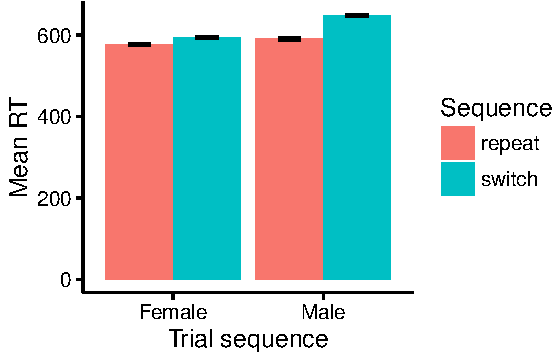
\includegraphics{Lab5_files/figure-latex/unnamed-chunk-2-1}

\begin{Shaded}
\begin{Highlighting}[]
\KeywordTok{ggplot}\NormalTok{(plot_means,}\KeywordTok{aes}\NormalTok{(}\DataTypeTok{x=}\NormalTok{Sequence, }\DataTypeTok{y=}\NormalTok{MeanRT, }\DataTypeTok{group=}\NormalTok{Gender,}\DataTypeTok{shape=}\NormalTok{Gender))+}
\StringTok{  }\KeywordTok{geom_line}\NormalTok{()+}
\StringTok{  }\KeywordTok{geom_point}\NormalTok{()+}
\StringTok{  }\KeywordTok{geom_errorbar}\NormalTok{(limits, }\DataTypeTok{width=}\NormalTok{.}\DecValTok{3}\NormalTok{)+}
\StringTok{  }\KeywordTok{theme_classic}\NormalTok{(}\DataTypeTok{base_size=}\DecValTok{12}\NormalTok{)+}
\StringTok{  }\KeywordTok{ylab}\NormalTok{(}\StringTok{"Mean RT"}\NormalTok{)+}
\StringTok{  }\KeywordTok{xlab}\NormalTok{(}\StringTok{"Trial sequence"}\NormalTok{)}
\end{Highlighting}
\end{Shaded}

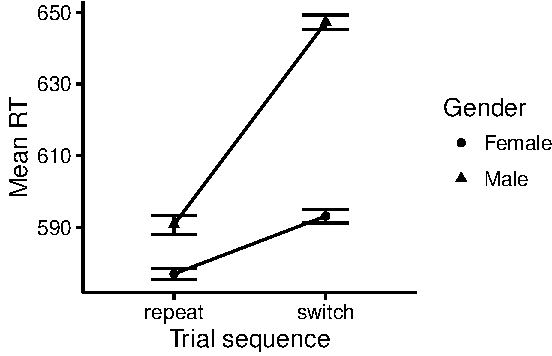
\includegraphics{Lab5_files/figure-latex/unnamed-chunk-3-1}

The graphs show that the switch costs (difference between repeat and
switch trials) is smaller for women and men. Which is good, because we
are simulating the data with this outcome in mind.

\subsection{Running the ANOVA}\label{running-the-anova}

The next step is to conduct an ANOVA. This design has two factors or
independent variables, gender and trial sequence. The gender variable is
between-subjects, and the trial sequence variable is within subjects.
So, we will run a 2 (Gender: Female vs.~Male) x 2 (trial sequence:
Repeat vs.~Switch) mixed design ANOVA with Gender as the betwen-subjects
factor, and trial sequence as the within-subjects factor.

\begin{Shaded}
\begin{Highlighting}[]
\KeywordTok{library}\NormalTok{(broom)}
\NormalTok{all_data$Subject<-}\KeywordTok{as.factor}\NormalTok{(all_data$Subject)}
\NormalTok{aov.out<-}\KeywordTok{aov}\NormalTok{(RT~Gender*Sequence+}\KeywordTok{Error}\NormalTok{(Subject/Sequence),all_data)}
\NormalTok{aov_summary<-}\KeywordTok{summary}\NormalTok{(aov.out)}
\KeywordTok{kable}\NormalTok{(}\KeywordTok{xtable}\NormalTok{(aov_summary),}\DataTypeTok{format=}\StringTok{"latex"}\NormalTok{)}
\end{Highlighting}
\end{Shaded}

\begin{tabular}{l|r|r|r|r|r}
\hline
  & Df & Sum Sq & Mean Sq & F value & Pr(>F)\\
\hline
Gender & 1 & 11458.225 & 11458.2250 & 22.10104 & 1.78e-04\\
\hline
Residuals & 18 & 9332.050 & 518.4472 & NA & NA\\
\hline
Sequence & 1 & 13140.625 & 13140.6250 & 38.47507 & 7.50e-06\\
\hline
Gender:Sequence & 1 & 4060.225 & 4060.2250 & 11.88813 & 2.87e-03\\
\hline
Residuals & 18 & 6147.650 & 341.5361 & NA & NA\\
\hline
\end{tabular}

\begin{Shaded}
\begin{Highlighting}[]
\NormalTok{mt<-}\KeywordTok{model.tables}\NormalTok{(aov.out,}\StringTok{"means"}\NormalTok{)}
\NormalTok{mt}
\end{Highlighting}
\end{Shaded}

\begin{verbatim}
## Tables of means
## Grand mean
##         
## 602.075 
## 
##  Gender 
## Gender
## Female   Male 
##  585.1  619.0 
## 
##  Sequence 
## Sequence
## repeat switch 
##  583.9  620.2 
## 
##  Gender:Sequence 
##         Sequence
## Gender   repeat switch
##   Female 577.1  593.2 
##   Male   590.8  647.2
\end{verbatim}

The above shows the ANOVA table and the means for the main effects and
interaction. We also conduct t.test comparisons to look at the switch
costs separately for men and women.

\begin{Shaded}
\begin{Highlighting}[]
\NormalTok{FemaleT<-}\KeywordTok{t.test}\NormalTok{(RT~Sequence,all_data[all_data$Gender==}\StringTok{"Female"}\NormalTok{,],}\DataTypeTok{paired=}\OtherTok{TRUE}\NormalTok{,}\DataTypeTok{var.equal=}\OtherTok{TRUE}\NormalTok{)}
\NormalTok{MaleT<-}\KeywordTok{t.test}\NormalTok{(RT~Sequence,all_data[all_data$Gender==}\StringTok{"Male"}\NormalTok{,],}\DataTypeTok{paired=}\OtherTok{TRUE}\NormalTok{,}\DataTypeTok{var.equal=}\OtherTok{TRUE}\NormalTok{)}
\NormalTok{FemaleT}
\end{Highlighting}
\end{Shaded}

\begin{verbatim}
## 
##  Paired t-test
## 
## data:  RT by Sequence
## t = -2.3034, df = 9, p-value = 0.04674
## alternative hypothesis: true difference in means is not equal to 0
## 95 percent confidence interval:
##  -31.9115634  -0.2884366
## sample estimates:
## mean of the differences 
##                   -16.1
\end{verbatim}

\begin{Shaded}
\begin{Highlighting}[]
\NormalTok{MaleT}
\end{Highlighting}
\end{Shaded}

\begin{verbatim}
## 
##  Paired t-test
## 
## data:  RT by Sequence
## t = -6.0205, df = 9, p-value =
## 0.0001975
## alternative hypothesis: true difference in means is not equal to 0
## 95 percent confidence interval:
##  -77.59196 -35.20804
## sample estimates:
## mean of the differences 
##                   -56.4
\end{verbatim}

\subsection{Writing up the results}\label{writing-up-the-results}

The next step is to interpret the results and write them up. Here is an
example write-up.

The mean reaction times for each subject in trial sequence condition
were submitted to a 2 (Gender: Female vs.~Male) x 2 (trial sequence:
Repeat vs.~Switch) mixed design ANOVA with Gender as the betwen-subjects
factor, and trial sequence as the within-subjects factor. Mean reaction
times in each condition collapsed across subjects are displayed in
Figure 1.

The main effect of gender was significant, F(1, 18) = 22.1, MSE =
518.45, p \textless{} 0. Women (585 ms) had faster mean reaction times
than men (619 ms).

The main effect of trials sequence was significant, F(1, 18) = 38.48,
MSE = 341.54, p \textless{} 0. Repeat trials (584) had faster mean
reaction times than switch trials (620).

Most important was the significant two-way interaction between gender
and trial sequence, F(1, 18) = 11.89, MSE = 341.54, p \textless{} 0.003.
We interpreted the interaction further by conducting the following
comparisons. Women showed a significant switch cost, t(9) = -2.3, p =
0.047, with faster mean reaction times for repeat (577) than switch
(593) trials. Men also showed a significant switch cost, t(9) = -6.02, p
= 0, with faster mean reaction times for repeat (591) than switch trials
(647). The presence of an interaction indicates that the size of the
switch cost for women was significantly smaller than the size of the
switch cost for men.








